\section{Experiments III: real data}\label{sec:real}

\subsection{Real account-level order flow}\label{sec:real-accounts}

Every result above is for simulated accounts. To see what the statistic does on real accounts we use two public data sets from a venue with an account identifier on every record, the Hyperliquid derivatives exchange. They are far from the Vietnamese market (a crypto perpetual-futures venue, dominated by automated accounts, with pseudonymous addresses that one operator may use in several copies), so the results are a stress test of the statistic, not an estimate for Vietnam. There are no manipulation labels.

\paragraph{Data.} \emph{Order submissions}: the Level-4 order data of \citet{albers2026} (Zenodo record 18184441, CC BY 4.0), first member of the December 2025 file for the SOL perpetual, 577,918 orders submitted by 1,909 accounts in 23.6 minutes of 1 December 2025; we use one record per order identifier and the side of the order, windows of 300 bins of 0.5 seconds (150 seconds; nine windows with 351 to 715 active accounts and 61,000 orders on average). \emph{Fills}: a public table of fills (account address, side, millisecond time) of a 91-minute slice of 5 June 2026 for the perpetual contracts HYPE, BTC and ETH, windows of 300 bins of one second (18 windows). Accounts with fewer than three records in a window are not tested.

\paragraph{Calibration on real flow.} Table~\ref{tab:realcal} gives the share of accounts with small $p$-values. On submissions, 28.5\% of accounts with at least three orders in a window have $p\le0.01$ for the signed statistic (33.4\% unsigned), against a nominal 1\%, and the share rises with activity: 6.6\% for accounts with 3 to 9 orders, 32.6\% for 10 to 99, 51.8\% for 100 or more; for accounts that trade on both sides it is 43.6\%. Netting buys against sells barely lowers the rate, unlike in the simulator: real market makers do not re-quote symmetrically but shift both quotes in the direction of the last price move, so their net flows are positively correlated (Proposition~\ref{prop:netting} covers the symmetric case only). The exchangeability condition of Proposition~\ref{prop:exact} is violated for a large share of the active accounts of this venue: they react to the same signals. The aggregate flow of the other accounts is also dominated by a few loud accounts: its variance per bin, divided by the median variance of a quiet account (3 to 15 orders in the window), gives an effective number of accounts $N_{\mathrm{eff}}\approx10^6$ (Section~\ref{sec:power}) against about 470 accounts, so that a ring of quiet accounts is nearly invisible unless it is loud. On fills the pattern is mechanical and different: the signed statistic flags almost nothing (0.0--0.03\%) and the unsigned one 15--17\%, because each trade appears twice, as the buy of one account and the sell of its counterparty in the same millisecond, so that the aggregate of the others contains the mirror image of every account's own flow. The test must be applied to submissions, not to executed trades.

\begin{table}[t]
\centering\footnotesize
\adjustbox{max width=\linewidth}{\begin{tabular}{llrrrrr}
\toprule
data & accounts & account-windows & unsigned, $p\le0.01$ & signed, $p\le0.01$ & unsigned, $p\le0.05$ & signed, $p\le0.05$ \\
\midrule
fills, BTC & all with $\ge3$ & 3765 & 0.156 & 0.000 & 0.298 & 0.000 \\
fills, ETH & all with $\ge3$ & 1930 & 0.166 & 0.000 & 0.308 & 0.000 \\
fills, HYPE & all with $\ge3$ & 3732 & 0.151 & 0.000 & 0.290 & 0.001 \\
order submissions, SOL & 3--9 submissions & 843 & 0.075 & 0.066 & 0.198 & 0.206 \\
order submissions, SOL & 10--99 & 645 & 0.332 & 0.326 & 0.457 & 0.437 \\
order submissions, SOL & $\ge100$ & 682 & 0.655 & 0.518 & 0.723 & 0.594 \\
order submissions, SOL & all with $\ge3$ & 2170 & 0.334 & 0.285 & 0.440 & 0.397 \\
order submissions, SOL & both sides & 1166 & 0.525 & 0.436 & 0.624 & 0.534 \\
\bottomrule
\end{tabular}
}
\caption{Share of accounts flagged on real account-level flow (accounts with at least three records in the window). Under the null of Proposition~\ref{prop:exact} the share would be at most the level}\label{tab:realcal}
\end{table}

\paragraph{A ring planted in real flow.} To measure power against the real background, we choose $K=12$ quiet real accounts (3 to 15 orders in the window) and add to each, at ten common bins of the window (each member jittered by at most one bin), $q$ buy orders; the other accounts' flow is unchanged. Table~\ref{tab:realplant} and Figure~\ref{fig:realacc} give catch@$B$ over 180 trials (nine windows, 20 draws each). With no planting ($q=0$) none of the chosen accounts reaches the top five. A ring of three orders per push is undetectable; at 30 orders per member and push (5.9\% of the orders of the window in total) it is in the top ten in none of the 180 trials although 41\% of its members have $p\le0.01$, because more than a quarter of all accounts have $p\le0.01$ for natural reasons and the ranking is filled by loud accounts; at 100 orders (19.5\% of the flow of the window) it is in the top five in 80\% of the trials (signed statistic), and at 300 in all. The dependence on the design is steep and in the direction of Proposition~\ref{prop:power}: catch@5 falls from 1.00 to 0.79 as the number of accounts rises from 100 to 468 (by dropping real accounts at random), it is 0 for a ring of four, 0.26 for eight and 1.00 for 16 accounts, and 0.22, 0.79 and 1.00 for three, ten and thirty pushes per window. A ring of 12 retail accounts that submits a few orders at each of ten moments would not be found in this venue by this statistic; a ring that makes up a fifth of the flow of a stock-window would be. Whether a Vietnamese stock has a background as loud as this one is the empirical question account-level data would settle, and the planted-ring audit is the way to measure it (Section~\ref{sec:discussion}).

\begin{figure}[t]
\centering
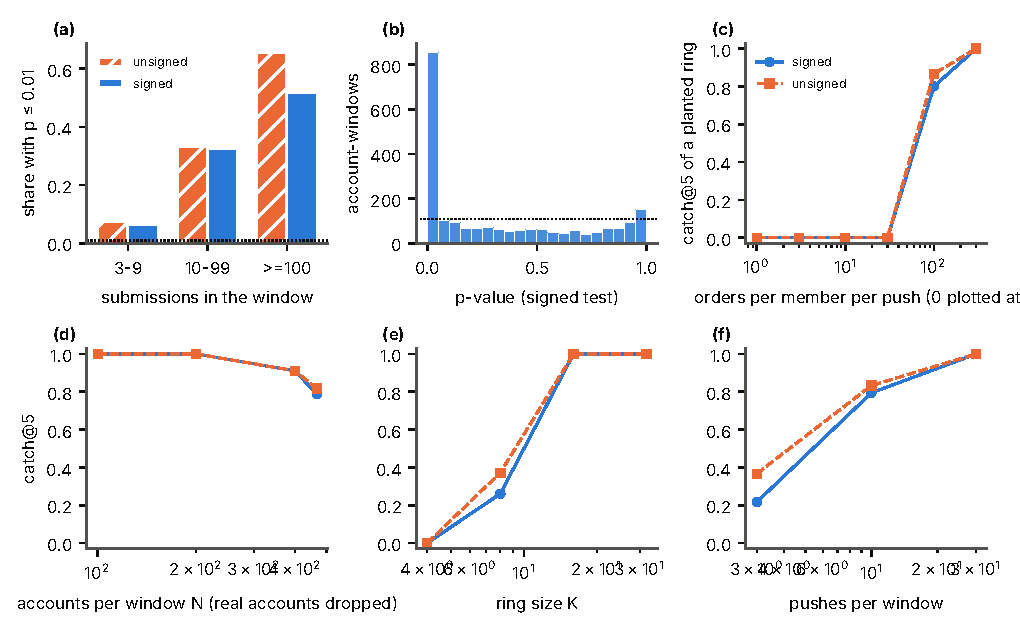
\includegraphics[width=\linewidth]{figures/real_accounts.pdf}
\caption{The coincidence test on real order submissions (SOL perpetual, 23.6 minutes). (a) Share of accounts with $p\le0.01$ by number of submissions in the window; dotted: nominal 1\%. (b) Histogram of signed-test $p$-values of accounts with at least three submissions; dotted: uniform. (c)--(f) catch@5 of a ring of 12 quiet real accounts planted at ten common moments per window, signed (solid) and unsigned (dashed), against the number of orders per member and push (c), the number of accounts (d), the ring size (e) and the number of pushes per window (f); unless varied, $q=100$ orders per push and the full set of accounts}\label{fig:realacc}
\end{figure}

\begin{table}[t]
\centering\scriptsize
\setlength{\tabcolsep}{3pt}
\adjustbox{max width=\linewidth}{\begin{tabular}{lrrrrrrrrr}
\toprule
sweep & $N$ & $K$ & orders per push & pushes & unsigned @5 & signed @1 & signed @5 & signed @10 & members with $p\le0.01$ \\
\midrule
orders per push & 468 & 12 & 0 & 10 & 0.00 & 0.00 & 0.00 & 0.00 & 0.09 \\
orders per push & 468 & 12 & 3 & 10 & 0.00 & 0.00 & 0.00 & 0.00 & 0.03 \\
orders per push & 468 & 12 & 10 & 10 & 0.00 & 0.00 & 0.00 & 0.00 & 0.06 \\
orders per push & 468 & 12 & 30 & 10 & 0.00 & 0.00 & 0.00 & 0.00 & 0.41 \\
orders per push & 468 & 12 & 100 & 10 & 0.87 & 0.59 & 0.80 & 0.89 & 1.00 \\
orders per push & 468 & 12 & 300 & 10 & 1.00 & 1.00 & 1.00 & 1.00 & 1.00 \\
accounts & 100 & 12 & 100 & 10 & 1.00 & 1.00 & 1.00 & 1.00 & 1.00 \\
accounts & 200 & 12 & 100 & 10 & 1.00 & 1.00 & 1.00 & 1.00 & 1.00 \\
accounts & 400 & 12 & 100 & 10 & 0.91 & 0.78 & 0.91 & 0.96 & 1.00 \\
accounts & 468 & 12 & 100 & 10 & 0.82 & 0.65 & 0.79 & 0.91 & 1.00 \\
ring size & 468 & 4 & 100 & 10 & 0.00 & 0.00 & 0.00 & 0.00 & 0.38 \\
ring size & 468 & 8 & 100 & 10 & 0.37 & 0.19 & 0.26 & 0.29 & 0.91 \\
ring size & 468 & 16 & 100 & 10 & 1.00 & 1.00 & 1.00 & 1.00 & 1.00 \\
ring size & 468 & 32 & 100 & 10 & 1.00 & 0.99 & 1.00 & 1.00 & 1.00 \\
pushes per window & 468 & 12 & 100 & 3 & 0.37 & 0.17 & 0.22 & 0.24 & 0.85 \\
pushes per window & 468 & 12 & 100 & 10 & 0.83 & 0.64 & 0.79 & 0.86 & 1.00 \\
pushes per window & 468 & 12 & 100 & 30 & 1.00 & 1.00 & 1.00 & 1.00 & 1.00 \\
\bottomrule
\end{tabular}
}
\caption{Planted ring among 12 quiet real accounts: catch@$B$ over 180 trials (nine windows, 20 draws), ranking by the signed statistic (unsigned at 5 for comparison), and share of members with $p\le0.01$. The sweep column names the factor that varies; the others are at $N=468$, $K=12$, 100 orders per push and 10 pushes}\label{tab:realplant}
\end{table}


\subsection{Documented enforcement cases on daily prices}\label{sec:cases}

\paragraph{Data and protocol.} Ten decisions of the State Securities Commission with exact dates of the conduct were collected from press reports quoting the decisions (Appendix~\ref{app:cases}; the decision documents were not opened). For every stock and date, using only data up to that date, we compute market-adjusted abnormal return, volume surge against the stock's own history, a round-trip statistic, the position of the close in the daily range, the count of days with moves of at least 6.5\%, and range expansion; stocks are ranked against each other on each date. The protocol, fixed before the cases were scored, is: a case stock is scored by the highest rank it reaches on any date in its period; two nulls are used, 300 random stocks over the same dates and 300 non-overlapping periods of the same length of the same stock; and we count the cases in which the stock is among the $B$ highest of its date at least once.

\paragraph{Results.} Table~\ref{tab:cases} gives the results. The market-adjusted abnormal return alone places 8 of the 10 cases in the daily top ten of about 1,360 scored stocks at some point of their period, against 15\% for random stocks over the same dates, and a case stock beats a random stock with probability 0.89 and the same stock at other times with probability 0.87. These are not stocks that rank high at all times. Combining six features, or an isolation forest on them, is no better than the single feature. Volume surge behaves differently in the two comparisons: against the same stock at other times it is informative (superiority 0.90, five of ten cases with $p<0.05$), against other stocks it is not (0.33), because other stocks have larger surges at some time; we therefore claim nothing new for the market-level detector. Table~\ref{tab:window} shows that the abnormal-return result is stable across window lengths of 10, 20 and 60 days (superiority over random stocks 0.87, 0.89, 0.85; over the same stock 0.78, 0.87, 0.89). The result says little about precision: periods are long (83 to 587 trading days), only ten cases are documented among thousands of price run-ups, and an unlabelled run-up is not an innocent one.

\begin{table}[t]
\centering\footnotesize
\adjustbox{max width=\linewidth}{\begin{tabular}{lrrrrrrr}
\toprule
detector & superiority & top 10 & chance & top 20 & chance & top 50 & chance \\
\midrule
market-adjusted abnormal return & 0.89 & 8/10 & 15\% & 10/10 & 27\% & 10/10 & 53\% \\
combined six-feature score & 0.78 & 6/10 & 22\% & 6/10 & 35\% & 10/10 & 58\% \\
isolation forest, same features & 0.78 & 7/10 & 21\% & 8/10 & 34\% & 9/10 & 54\% \\
round trip (run-up, retracement) & 0.70 & 9/10 & 76\% & 10/10 & 81\% & 10/10 & 90\% \\
volume surge & 0.33 & 0/10 & 3\% & 0/10 & 5\% & 0/10 & 13\% \\
\bottomrule
\end{tabular}
}
\caption{Ten documented cases scored against about 1,360 stocks (20-day window). Superiority is the probability that a case stock beats a random stock (0.5 is chance); ``top $B$'' counts cases in which the stock reached the daily top-$B$ list at some date of its period; ``chance'' is the same share for random stocks.}\label{tab:cases}
\end{table}

\begin{table}[t]
\centering\footnotesize
\adjustbox{max width=\linewidth}{\begin{tabular}{llrrr}
\toprule
window (days) & detector & superiority vs random stocks & superiority vs same stock & cases in top 10 / 10 \\
\midrule
10 & abnormal return & 0.87 & 0.78 & 9 \\
10 & combined score & 0.69 & 0.70 & 5 \\
10 & volume surge & 0.33 & 0.88 & 0 \\
20 & abnormal return & 0.89 & 0.87 & 8 \\
20 & combined score & 0.79 & 0.86 & 6 \\
20 & volume surge & 0.33 & 0.90 & 0 \\
60 & abnormal return & 0.85 & 0.89 & 3 \\
60 & combined score & 0.77 & 0.88 & 3 \\
60 & volume surge & 0.28 & 0.79 & 0 \\
\bottomrule
\end{tabular}
}
\caption{Sensitivity to the window length. Superiority against random stocks and against the same stock at other times; number of cases in the daily top ten.}\label{tab:window}
\end{table}

\paragraph{Event time.} Figure~\ref{fig:cases} aligns the ten cases at the first day of their documented period. The cumulative market-adjusted return of the case stocks is flat before the period and rises through it (mean $+0.29$ twenty days after the start and $+0.42$ after sixty), the mean percentile of the abnormal-return score rises from 0.39 sixty days before to 0.78 twenty days after, and the percentile of the volume-surge score does not rise consistently (0.34 at day $-60$, 0.41 at day 20, 0.28 at day 60), which is the reading of Table~\ref{tab:cases} in time: the price runs up on ordinary volume.

\begin{figure}[t]
\centering
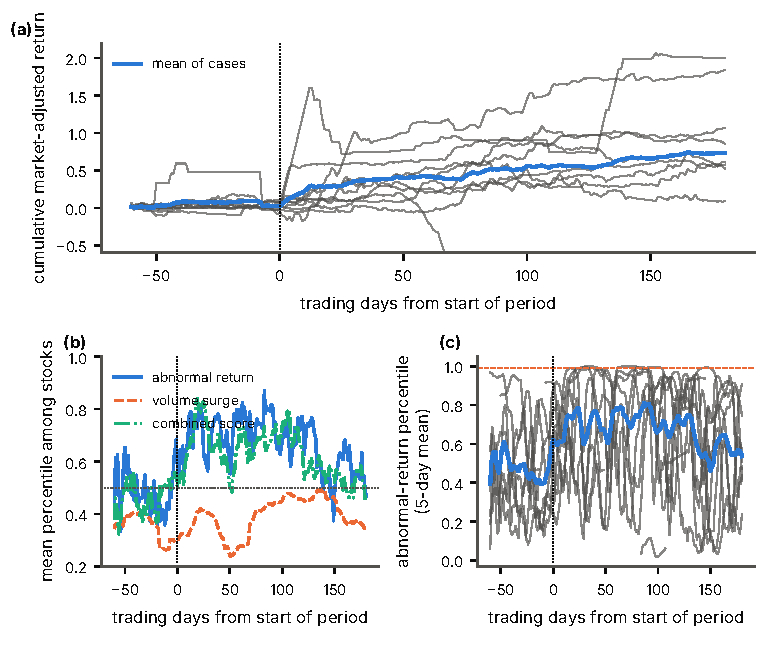
\includegraphics[width=\linewidth]{figures/cases.pdf}
\caption{The ten documented cases in event time (day 0 is the first day of the documented period). (a) Cumulative market-adjusted log return since day $-60$: individual cases (grey) and mean (blue). (b) Mean cross-sectional percentile among all stocks of three scores computed from data up to each day (20-day windows). (c) Percentile of the abnormal-return score, 5-day moving average, individual cases (grey) and mean (blue); dashed line: the 99th percentile}\label{fig:cases}
\end{figure}

\paragraph{Case stocks and the daily band.} Table~\ref{tab:casestats} compares the case stocks with the market and counts days within 0.5 points of the daily ceiling. The stocks are ordinary (median daily volatility 1.75\% in the year before against 2.46\% for HOSE stocks), and the band is reached in their manipulation periods: five ceiling days at the median, and runs of up to 12 days. This differs from the simulated ring, whose price displacement of about 0.5\% never reaches the band. The band could matter for a manipulator who ratchets the price over days; our simulated rings do not, so the finding that the band has no effect is a statement about rings of the size we simulate, not about all manipulation.

\begin{table}[t]
\centering\footnotesize
\adjustbox{max width=\linewidth}{\begin{tabular}{llrrrrrrr}
\toprule
stock & exchange & days & pre-period vol. (\%) & vol. in period (\%) & zero-return share & log price change ($\times100$) & ceiling days & longest run \\
\midrule
FIR & HOSE & 109 & 1.63 & 1.84 & 0.02 & +38 & 0 & 0 \\
SJS & HOSE & 192 & 2.32 & 2.34 & 0.13 & +49 & 10 & 3 \\
PDR & HOSE & 83 & 1.94 & 3.84 & 0.07 & -119 & 4 & 3 \\
PSH & unknown & 319 & 1.75 & 3.45 & 0.45 & -12 & 26 & 3 \\
AGG & HOSE & 514 & 1.29 & 1.90 & 0.13 & +35 & 7 & 1 \\
CRC & HOSE & 106 & 1.36 & 2.65 & 0.18 & +73 & 5 & 1 \\
GKM & HNX & 125 & 1.62 & 3.77 & 0.32 & +157 & 1 & 1 \\
PAS & UPCOM & 491 & 3.37 & 3.54 & 0.10 & -87 & 0 & 0 \\
HCI & unknown & 146 & 6.78 & 6.17 & 0.81 & +183 & 21 & 12 \\
\bottomrule
\end{tabular}
}
\caption{Case stocks: daily volatility and zero-return share in the year before the period, volatility during it, price change over the period, days within 0.5 points of the daily ceiling and the longest run of such days.}\label{tab:casestats}
\end{table}

\subsection{Telegram-organised pump events on tick data}\label{sec:pump}

We use a public archive of 701 pump events with trades from about 24 hours before the pump time to shortly after (Appendix~\ref{app:calib}). The files hold side, price and amount, with no account identifiers, so the coincidence test cannot be applied. For each event, standardised volume and buy imbalance over rolling ten-minute windows are measured against the same coin's first 20 hours. Figure~\ref{fig:pump} shows accumulation: mean standardised volume rises from 0.19 (4 to 3 hours before) to 0.71 (last ten minutes), and buy imbalance from 0.03 to 0.23, with intervals excluding zero, and both jump at the pump. This supports the accumulate--push structure of the simulated ring. It does not give early warning: with the alarm rate in the background set to 0.05 per coin-hour, only 6.0\% of events raise an alarm in the last hour before the pump (8.3\% at 0.1 and 16.4\% at 0.25 per coin-hour; median lead 7 to 15 minutes when it fires).

\begin{figure}[t]
\centering
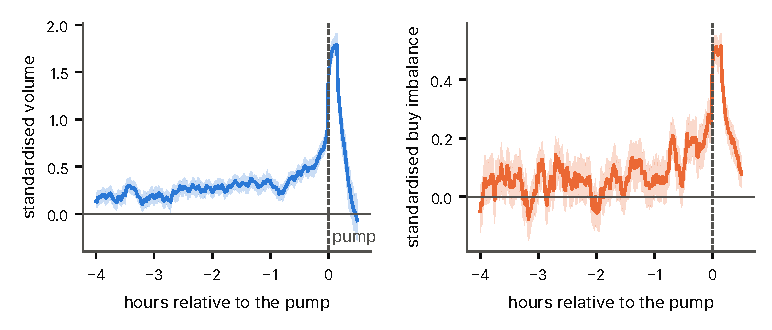
\includegraphics[width=0.85\linewidth]{figures/pump.pdf}
\caption{Standardised volume and buy imbalance of 701 pump events around the pump time (mean and 95\% bootstrap interval over events)}\label{fig:pump}
\end{figure}


